\section{Mapserver}
MapServer adalah program penggambar data geografis open source yang ditulis
dalam bahasa C \cite{akbar2011peningkatan}. Atau sebuah aplikasi freeware dan open source yang dapat menampilkan data spasial (peta) pada web. Aplikasi ini dikembangkan pertama kali oleh Universitas Minesotta, Amerika Serikat dalam projek ForNet yang merupakan sebuah projek untuk manajemen sumber daya alam yang disponsori NASA. kemudian dikembangkan projek TerraSIP sebagai manajemen data lahan. Karena sifatnya terbuka atau open source, pengembangan MapServer dilakukan oleh banyak negara.

 MapServer juga merupakan sebuah aplikasi yang berbasis Open Source yang digunakan untuk merender data geografis yang dibuat menggunakan bahasa pemograman C. Dengan menggunakan MapServer, memungkinkan terciptanya sebuah peta geografis yaitu peta-peta yang dapat mengarahkan pengguna.

MapServer adalah salah satu proyek pendiri yayasan OSGeo, dan dikelola oleh semakin banyak pengembang (mendekati 20) dari seluruh dunia. Ini didukung oleh beragam kelompok organisasi yang mendanai perangkat tambahan dan pemeliharaan, dan dikelola di dalam OSGeo oleh Komite Pengarah Proyek MapServer yang terdiri dari pengembang dan kontributor lainnya. Semua kode sumber tersedia secara terbuka melalui GitHub.

Mekanisme mapserver yaitu membuat layer-layer yang berisi berupa tampilan peta. Contohnya, layer peta Negara Indonesia, layer batas provinsi di Indonesia, layer batas kabupaten di Indonesia, layer titik-titik, dll. Ilustrasi layer berupa tampilan tersebut adalah sebagai berikut: angka paling rendah merupakan layer paling atas dan angka paling tinggi merupakan layer yang paling bawah.

Kekurangan mapserver adalah penggunaan dan konfigurasi mapfile yang cukup sulit untuk pemula. Developer harus melihat dan mengatur layer dengan cara mengcoding mapfile tersebut. Kemudian jika data GIS tersimpan dalam database peta. Mapserver perlu diatur koneksinya. Hal ini cukup sulit karena informasi host, username, password, port, dan database ditampilkan di mapfile tanpa ada proses enkripsi. Solusinya dengan menjaga agar mapfile ini tidak bisa diakses dari luar server.

Map Server bekerja beriringan dengan aplikasi web server. Web Server menerima request peta melalui MapServer, lalu MapServer mengenerate request terhadap peta lalu mengirimkannya ke web server seperti gambar dibawah ini.
\begin{figure}[ht]
	    \centerline{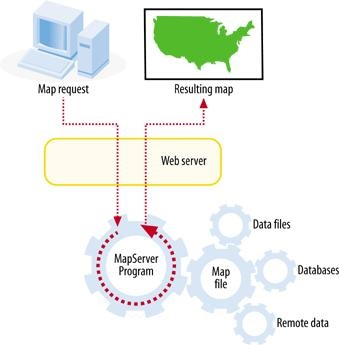
\includegraphics[width=0.50\textwidth]{figures/gambar5.JPG}}
	    \caption{Diagram operasi standar pada MapServer}
		\label{gambar5}
		\end{figure}
Fungsi utama dari MapServer yaitu untuk melakukan pembacaan data dari berbagai sumber dan menempatkannya kedalam layer-layer secara bersamaan yang kemudian menjadi file graphic.

Mapserver menghasilkan keluaran berupa file graphic berdasarkan masukan yang diberikan oleh user. Komponen kuncinya adalah MapServer executable yang terdiri dari CGI program, file peta, sumber data dan output gambar. Seperti pada gambar dibawah ini semua komponen bekerja bersama-sama, setelah user melakukan request/perminataan maka CGI akan mengakses file peta, menggambarkan informasi yang didapat dari sumber data dan kembali menampilkannya pada peta.

\subsection{Pengertian MS4W}
MapServer for Windows (MS4W) adalah suatu packet software untuk mempermudah pengguna dalam menginstalasi MapServer pada platform OS Microsoft Windows. Tujuannya adalah untuk mempermudah semua user, terhindar dari segala bagian kecil yang rumit dalam mempersiapkan lingkungan kerja yang dibutuhkan oleh MapServer pada lingkungan Microsoft Windows. Software ini juga merupakan suatu cara yang bagus dalam memaketkan kemudian mendistribusikan aplikasi-aplikasi MapServer kepada pihak manapun.

MS4W dilengkapi dengan berbagai modul tambahan yang mempermudah kita membangun dan mengadministrasi sistem WebGIS. Antara lain : MapLab, KaMap, Chameleon, dan lain-lain. MapLab digunakan untuk mempermudah kita membuat file konfigurasi MapServer ( *.map ) pada aplikasi WebGIS yang kita kembangkan. Sedang Chameleon adalah framework yang menyediakan berbagai class dan method yang mempermudah kita membangun interface aplikasi WebGIS yang kita kembangkan, seperti menambahkan fitur zoom, pan, dsb. Informasi mengenai MS4W, MapLab dan Chameleon dapat diperoleh di situs www.maptools.org. Di situs tersebut di dalamnya sudah terdapat aplikasi Apache Web Server, PHP, Map Server dan berbagai library yang diperlukan untuk membangun sistem WebGIS. Terdapat dua versi MS4W yang dapat didownload, versi 1.x dan versi 2.x. Akan tetapi Apabila kita akan menggunakan framework chameleon, lebih bagus pilih MS4W versi 1.x (versi 1.6) karena Chameleon belum mendukung penuh PHP5 pada paket MS4W versi 2.x.

\begin{table}[h]
\caption{Paket dasar M4SW}
\centering
\begin{tabular}{cc}
\hline
1&Webserver Apache\\
\hline
2&PHP\\
\hline
3&MapServer CGI\\
\hline
4&PHP/Mapscript\\
\hline
5&Program utiliti (pustaka) GDAL dan OGR\\
\hline
6&Program utiliti MapServer (shp2img, legend, scalebar, sortshp, sym2img, shptree, dan tile4ms)\\
\hline
7&Ekstensi OGR/PHP\\
\hline
8&OWTChart\\
\hline
\end{tabular}
\end{table}

\subsection{Cara Instalasi Mapserver}
\begin{enumerate}
\item
Download Mapserver atau disingkat MS4W di http://mapserver.org/download.html
\begin{figure}[ht]
	    \centerline{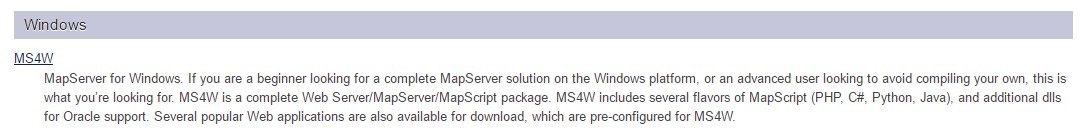
\includegraphics[width=0.50\textwidth]{figures/gambar1.JPG}}
	    \caption{Download MS4W}
		\label{gambar1}
		\end{figure}
\item
Setelah di download jalankan setupnya, disini saya menggunakan port 2000 karena port default 80 sudah dipakai oleh xampp
\begin{figure}[ht]
	    \centerline{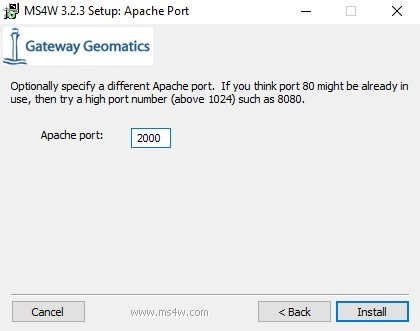
\includegraphics[width=0.50\textwidth]{figures/gambar2.JPG}}
	    \caption{Port 2000}
		\label{gambar2}
		\end{figure}
\item
Lalu tunggu instalasi sampai selesai
\begin{figure}[ht]
	    \centerline{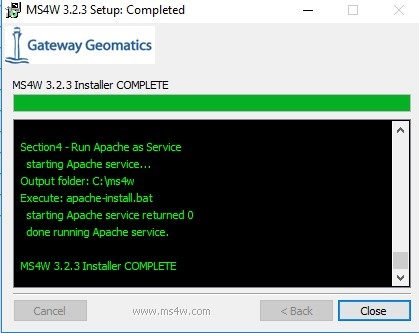
\includegraphics[width=0.50\textwidth]{figures/gambar3.JPG}}
	    \caption{Selesai}
		\label{gambar3}
		\end{figure}
\item
Setelah proses selesai silahkan buka browser favorit anda, kemudian ketikkan http://localhost:2000 di kotak isian URL.
\item
Jika anda melihat tampilan home MAPSERVER atau MS4W proses instalasi anda berhasil.
\begin{figure}[ht]
	    \centerline{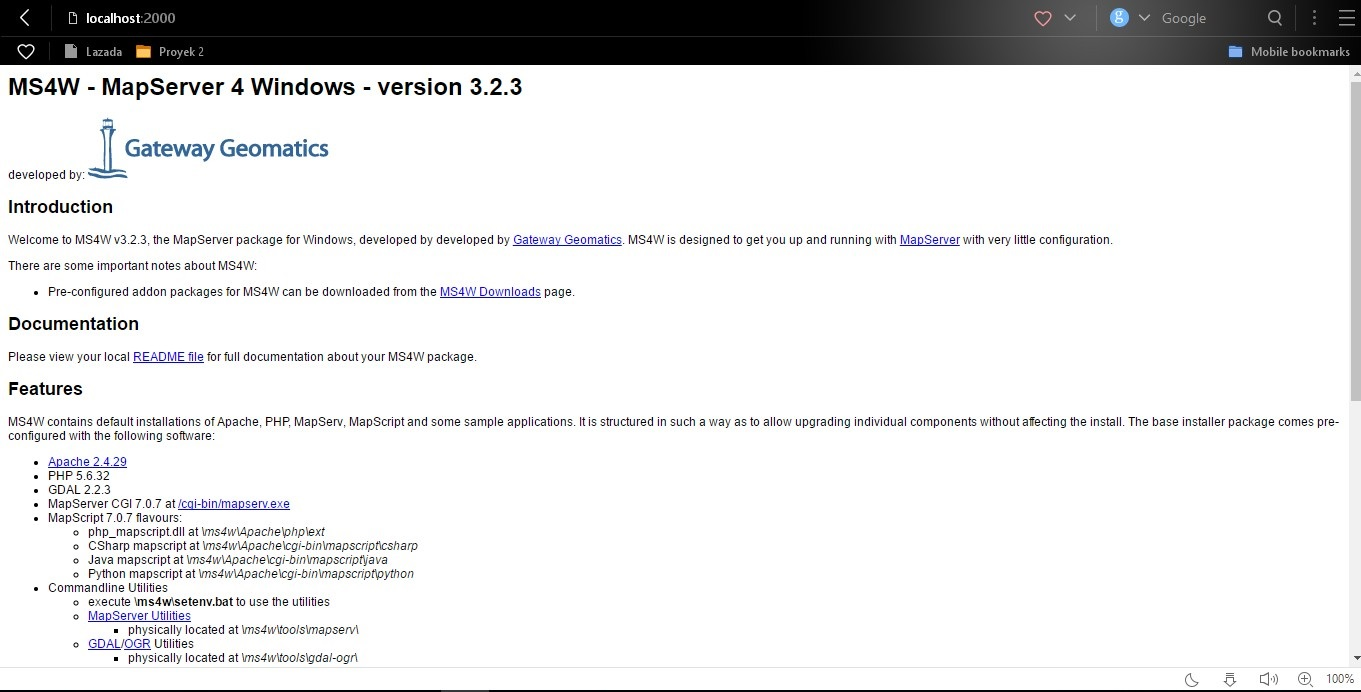
\includegraphics[width=0.50\textwidth]{figures/gambar4.JPG}}
	    \caption{Tampilan MS4W}
		\label{gambar4}
		\end{figure}
\end{enumerate}


\subsection{Arsitektur}
\begin{figure}[ht]
	    \centerline{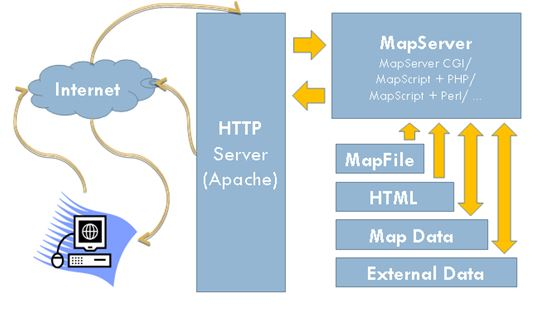
\includegraphics[width=0.50\textwidth]{figures/gambar6.JPG}}
	    \caption{Arsitektur}
		\label{gambar6}
		\end{figure}
Pada sistem aplikasi ini, browser (client) mengirimkan request (melalui jaringan internet/intranet) ke web server dalam bentuk request terkait spasial (lokasi[x,y] click kursor, status [on/off] layer yang akan dimunculkan, dsb).
Kemudian oleh web server, request terkait spasial ini dikirim ke server aplikasi (yang dibangun dengan menggunakan pemograman script yang telah tersedia) dan Mapserver (program CGI). Setelah itu, Mapserver akan membaca mapfile, data peta, dan data eksternal (jika ada dan memang diperlukan).
Setelah itu, gambar akan dikirim ke web server dan akhirnya browser milik client. Arsitektur Mapserver cenderung bercirikan thin-client.

Untuk dapat menjalankan dan menampilkan peta yang dihasilkan oleh MapServer, diperlukan dua file yaitu Map File dan HTML File. Map file berisikan konfigurasi penyajian peta yang ditulis dalam bahasa dan syntax tersendiri. Informasi itu kemudian diolah dan disajikan oleh program MapServer. 
Sedangkan file HTML digunakan untuk melakukan format penyajian hasil (peta). File HTML dapat berupa HTML biasa atau template yang disisipi syntax MapServer ataupun PHP/MapScript.

\begin{figure}[ht]
	    \centerline{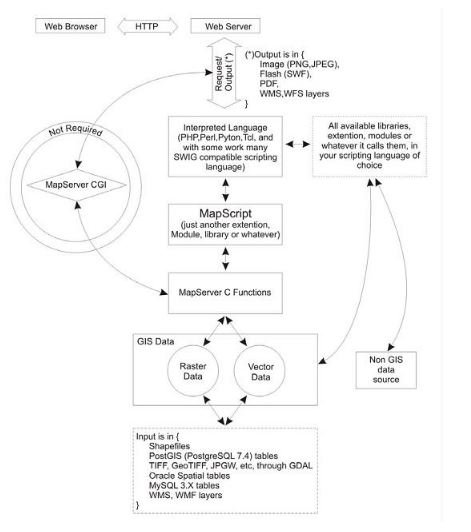
\includegraphics[width=0.50\textwidth]{figures/gambar7.JPG}}
	    \caption{Arsitektur}
		\label{gambar7}
		\end{figure}
		
Sebuah Map file harus memiliki komponen-komponen utama seperti images, data file berupa data vector maupun data raster yang akan ditampilkan oleh komponen layer.

\begin{figure}[ht]
	    \centerline{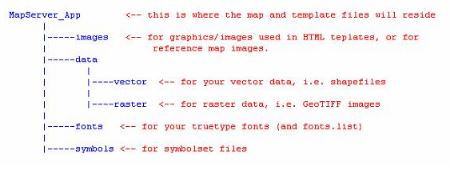
\includegraphics[width=0.50\textwidth]{figures/gambar8.JPG}}
	    \caption{Arsitektur}
		\label{gambar8}
		\end{figure}

\subsection{Arsitektur Dasar Aplikasi MapServer}
Map File - file konfigurasi teks terstruktur untuk aplikasi MapServer Anda. Ini mendefinisikan area peta Anda, memberi tahu program MapServer tempat data Anda berada dan di mana menampilkan gambar.
Data Geografis - MapServer dapat memanfaatkan banyak jenis sumber data geografis. Format defaultnya adalah format ESRI Shape.
HTML Pages - antarmuka antara pengguna dan MapServer. Mereka biasanya duduk di root Web. Dalam bentuknya yang paling sederhana, MapServer dapat dipanggil untuk menempatkan gambar peta statis pada halaman HTML. Untuk membuat peta interaktif, gambar ditempatkan dalam bentuk HTML pada halaman.
MapServer CGI - File biner atau executable yang menerima permintaan dan mengembalikan gambar, data, dan lain-lain. Ini ada di direktori cgi-bin atau script dari server web.
Web / HTTP Server - menyajikan halaman HTML saat dilanda browser pengguna.

\subsection{Kebutuhan Hardware}
MapServer berjalan di Linux, Windows, Mac OS X, Solaris, dan banyak lagi. Untuk mengkompilasi atau menginstal beberapa program yang diperlukan, Anda mungkin memerlukan hak administratif atas mesin. Orang biasanya mengajukan pertanyaan tentang spesifikasi perangkat keras minimum untuk aplikasi MapServer, namun jawabannya benar-benar spesifik untuk aplikasi individual. Untuk tujuan pengembangan dan pembelajaran, mesin yang sangat minim akan bekerja dengan baik. Untuk penyebaran, Anda ingin menyelidiki Optimalisasi segala sesuatu mulai dari data Anda hingga konfigurasi server.

\subsection{Kebutuhan Software}
Anda memerlukan server Web (HTTP) yang berfungsi dan dikonfigurasi dengan benar, seperti Apache atau Microsoft Internet Information Server, pada mesin tempat Anda menginstal MapServer.
Jika Anda menggunakan mesin Windows, dan Anda tidak menginstal server web, sebaiknya gunakan MS4W, yang akan menginstal server web pra-konfigurasi, MapServer, MapCache, PHP, TinyOWS, dan banyak lagi utilitas lainnya. Pengguna Windows secara opsional dapat memeriksa installer OSGeo4W juga.

\subsection{Pemahaman Pembelajaran Aplikasi MapServer}
Selain belajar bagaimana berbagai komponen aplikasi MapServer bekerja sama dan mempelajari sintaks Map File, membangun aplikasi dasar memerlukan beberapa pemahaman dan kemampuan konseptual di beberapa bidang keahlian.
Anda harus dapat membuat atau setidaknya memodifikasi halaman HTML dan memahami bagaimana bentuk HTML bekerja. Karena tujuan utama aplikasi MapServer adalah membuat peta, Anda juga perlu memahami dasar-dasar data geografis dan kemungkinan, memetakan proyeksi. Sebagai aplikasi Anda mendapatkan lebih kompleks, keterampilan di SQL, DHTML / Javascript, Java, database, ekspresi, kompilasi, dan scripting mungkin sangat berguna.

\subsection{Fitur-fitur yang ditawarkan MapServer :}
 \begin{enumerate}
\item Format Vektor : ESRI, shapefile, ESRI ArcSDE.
\item Format Raster : TIFF / GeoTIFF, GIF, PNG, ERDAS, JPEG, EPPL7.
\item Quadtree spatial indexing untuk shapefile.
\item Dapat sepenuhnya dikostumisasi untuk menghasilkan hasil yang diinginkan.
\item Pemilihan fitur menggunakan item/nilai, titik, area atau fitur lainnya.
\item Mendukung TrueType Font.
\item Mendukung OpenGIS.
\item Mendukung penggabungan data raster dan vector.
\item Legenda dan skala yang otomatis.
\item Mendukung pengembangan peta tematik online.
\item Pelabelan fitur.
\item Konfigurasi dapat dilakukan secara online.
\item Proyeksi dapat dilakukan secara online.
\end{enumerate}
Saat ini, selain dapat mengakses MapServer sebagai program CGI, kita juga dapat mengakses MapServer sebagai modul MapScript, dengan berbagai bahasa script  yaitu PHP, Perl, Python ataupun Java. Akses fungsi¬fungsi MapServer dengan menggunakan script akan lebih memudahkan dalam pengembangan aplikasi. Pengembang juga dapat memilih bahasa yang paling mudah digunakan.

\subsection{Optimalisasi Data}
Organisasi data setidaknya sama pentingnya dengan konfigurasi perangkat keras dalam mengoptimalkan aplikasi MapServer untuk kinerja. MapServer cukup efisien dalam hal ini, namun dengan mengurangi jumlah pemrosesan yang perlu dilakukan pada saat permintaan pengguna, Anda dapat meningkatkan kinerja. Berikut adalah beberapa aturannya:
\begin{enumerate}
\item Indeks Data Anda - Dengan membuat indeks spasial untuk dataset Shape Anda menggunakan shptree. Indeks spasial juga harus dibuat untuk database sadar spasial seperti PostGIS dan Oracle Spatial.

\item Tile Your Data - Idealnya, data Anda akan 'diiris' menjadi beberapa potongan ukuran yang akan ditampilkan. Ada overhead yang tidak perlu saat mencari melalui dataset Shape besar atau gambar yang hanya akan Anda tampilkan di area kecil. Dengan memecah data menjadi ubin dan membuat indeks genteng, MapServer hanya perlu membuka dan mencari file data yang diminati. Kumpulan data dapat dipecah menjadi ubin yang lebih kecil dan kemudian kumpulan data tileindex Shape dapat dibuat menggunakan utilitas tile4ms. Kumpulan data tileindex untuk file raster juga dapat dibuat.

\item Pra-Klasifikasi Data Anda - MapServer memungkinkan penggunaan EXPRESSION yang cukup kompleks untuk mengklasifikasikan data. Namun, menggunakan ekspresi logis dan reguler lebih banyak resource intensive daripada perbandingan string. Untuk meningkatkan efisiensi, Anda bisa membagi data Anda ke kelas lebih awal, membuat field untuk digunakan sebagai CLASSITEM dan mengisinya dengan nilai sederhana yang mengidentifikasi kelas, seperti 1,2,3, atau 4 untuk empat data kelas. set. Anda kemudian bisa melakukan perbandingan string sederhana untuk kelas EXPRESSION.

\item Pra-Proses Gambar Anda - Lakukan pemrosesan intensif sumber daya di depan. Lihat referensi Raster Data untuk info lebih lanjut.

\item Generalisasi untuk Ikhtisar - buat lapisan data yang lebih sederhana dan umum untuk ditampilkan pada skala kecil, lalu gunakan lapisan bergantung skala menggunakan LAYER MINSCALE dan LAYER MAXSCALE untuk menampilkan lapisan data yang lebih terperinci saat pengguna memperbesar. Konsep yang sama berlaku untuk gambar.
Lihat juga Optimalisasi
\end{enumerate}

\subsection {Membuat MapFile (Satu Layer)}
\begin {enumerate}
\item Buatlah folder baru dengan nama latihan di direktori apps yang ada di dalam folder
ms4w(dalam contoh ini folder ms4w berada di driver C:, sehingga nanti akan didapatkan path c:ms4w-apps-latihan). 

\item Copy data peta dan file pendukungnya (sebelumnya kita download terlebih dahulu, yang kita pakai adalah peta indonesia) ke dalam folder latihan tersebut

\item Buat folder map di folder latihan yang sebelumnya sudah dibut. Lalu buat sebuah mapfile sederhana dengan nama latihan01.map di direktori latihan/map. Mapfile ini akan digunakan untuk menampilkan sebuah layer (layer “Proponsi”) peta di layar web browser kita
\begin{figure}[ht]
	    \centerline{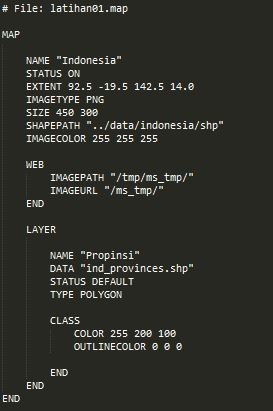
\includegraphics[width=0.50\textwidth]{figures/gambar9.JPG}}
	    \caption{File ekstensi *.map}
		\label{gambar9}
		\end{figure}

\item Untuk memunculkannya ketik di URL web browser seperti ini:
\begin{figure}[ht]
	    \centerline{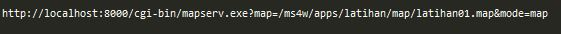
\includegraphics[width=0.50\textwidth]{figures/gambar10.JPG}}
	    \caption{URL}
		\label{gambar10}
		\end{figure}

\item Dan untuk hasilnya seperti ini
\begin{figure}[ht]
	    \centerline{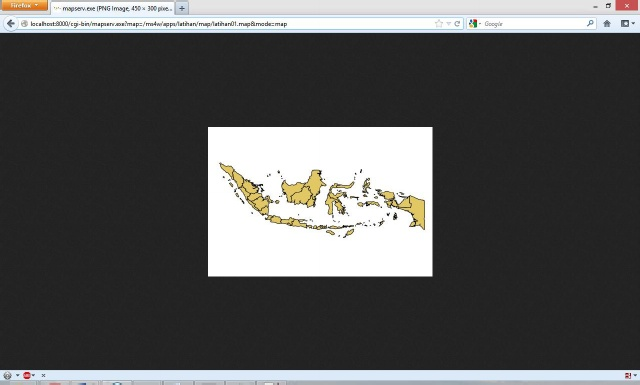
\includegraphics[width=0.50\textwidth]{figures/gambar11.JPG}}
	    \caption{Hasil Mapserver}
		\label{gambar11}
		\end{figure}
\end{enumerate}
